
\section{Decision Trees}

\textit{Decision Trees} are a versatile Machine Learning algorithm, that can outperform both classification and regression tasks,
and even multioutput tasks. This algorithm is very powerful, and is capable of fitting very complex datasets. Decision Trees
are also the fundamental building blocks of a Random Forest algorithm (Covered next section), which is one of the most 
powerful machine learning algorithms available today. \\

\noindent
In this section, we will cover how to train, visualize, and make predictions with Decision Trees (Using both Regression and 
classification).

\subsection{Training and Visualize a Decision Tree}

One of the easiest ways to understand \textit{Deicision Trees} is to build one and take a look how it makes predictions. Below
will be some code that trains a \mintinline{python}{DecisionTreeClassifier} on the iris dataset in Scikit-Learn:

\begin{minted}{python}
from sklearn.datasets import load_iris
from sklearn.tree import DecisionTreeClassifier

iris = load_iris()
X = iris.data[:, 2:] # Petal length and width
y = iris.target

tree_clf = DecisionTreeClassifier(max_depth=2, random_state=42)
tree_clf.fit(X, y)    
\end{minted}

\noindent
After running this code we can then visualize the Decision Tree by a graph format shown below:

\begin{center}
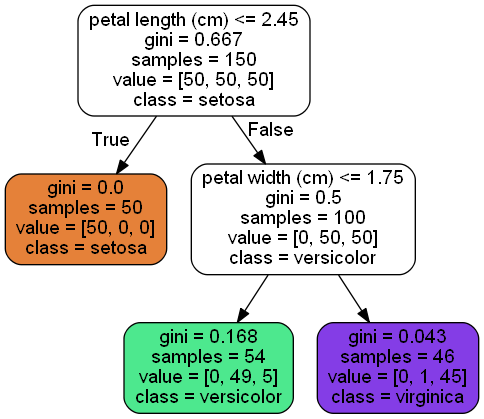
\includegraphics[scale=0.45]{Images/iris_tree.png}
\end{center}

\subsection{Making Predictions}

From the tree above we can show a logical process to classifying an iris flower. \\

\noindent
For example, lets say that we find an iris flower and we want to classify it, the steps will be as follows:

\begin{itemize}
    \item First we start at the \textit{root node} (depth 0, at the top): this node asks whether the flower's petal length is smaller than 
    2.45 cm.
    \item Second, if it is, then we move down to the root's left child node (depth 1, left)
    \item Third, we notice that in this case, this is a \textit{leaf node} (i.e., does not have any child nodes), so it is able to predict 
    the class of the iris. Which in this case, case classifies the iris flower as an \textit{iris setosa}
\end{itemize}

\noindent
**Note:** One of the great qualities about Decision Trees is that they require very little data preparation. I.e., they do not require 
feature scaling or centering at all. \\

\noindent
Node's Attributes:

\begin{itemize}
    \item \mintinline{python}{samples} attribute counts how many training instances it applies to. For example, 100 training instances
    have a petal length greater than 2.45 cm (depth 1, right), and of those 100, 54 have a petal width smaller than 1.75 cm 
    (depth 2, left). 
    \item \mintinline{python}{value} attribute tells us how many training isntances of each class this node applies to: for example, 
    the bottom-right node applies to 0 \textit{iris setosa}, 1 \textit{iris versicolor}, and 45 \textit{iris virginica}.
    \item \mintinline{python}{gini} attribute measures the \textit{impurity}: a node is "pure" (\mintinline{python}{gini=0}) if all 
    training instances it applies to belong to the same class. For example, since the depth-1 left node applies to only 
    \textit{iris setosa} training instances, it is pure and its gini score is 0. 
\end{itemize}

\noindent
Below will be the equation to compute the Gini Score:

$$G_{i} = 1 - \sum_{k=1}^{n} p_{i,k}^{2}$$

\noindent
In the equation above, $p_{i,k}$, is the ratio of class \mintinline{python}{k} instances among the training instances in the 
$i^{th}$ node \\

\noindent
Where we can compute the depth-2 left node gini attribute by the following: 

$$1 - \left(\frac{0}{54}\right)^{2} - \left(\frac{49}{54}\right)^{2} - \left(\frac{5}{54}\right)^{2} \approx 0.168$$ \\

\noindent
We can also view the decision boundaries of this Decision Tree through plots made in \mintinline{python}{matplotlib}. 

\begin{center}
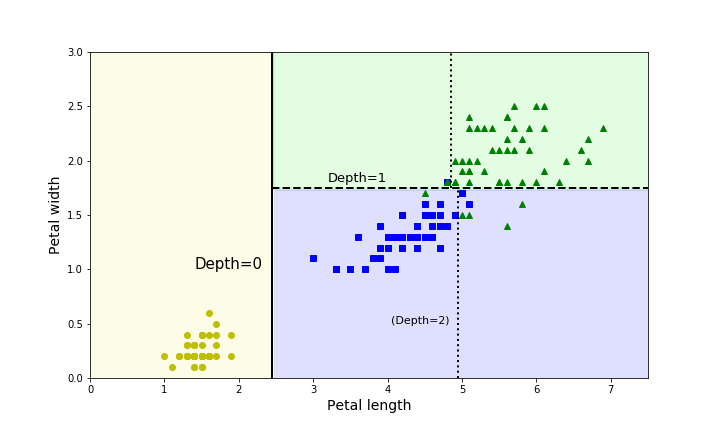
\includegraphics[scale=0.45]{Images/DecisionTreePlot.png}
\end{center}

\subsection{Estimating Class Probabilities}

A Decision Tree can also estimate the probability that an instance belongs to a particular class $k$. First it traverses the tree to find 
the leaf node for this instance, and then it returns the ration of training instances of class $k$ in this node. For example, suppose you 
have found a flower whose petals are 5 cm long and 1.5 cm wide. The corresponding leaf node is the depth-2 left node, so the Decision Tree 
should output the following probabilities: 0\% for Iris setosa ($\frac{0}{54}$), 90.7\% for Iris versicolor ($\frac{49}{54}$), and 9.3\% 
for Iris virginica ($\frac{5}{54}$). And if you ask it to predict the class, it should output Iris versicolor (class 1) because it has the 
highest probability. \\ 

\noindent
We can verify this with the following code:

\begin{minted}{python}
tree_clf.predict_proba([[5, 1.5]])
'''
Output:
array([[0.        , 0.90740741, 0.09259259]])
'''

tree_clf.predict([[5, 2.5]])
'''
Output:
array([1])
'''    
\end{minted}

\subsection{The CART Training Algorithm}

Scikit-Learn uses the \textit{Classification and Regresstion Tree} (CART) algorithm to train Decision Trees. This algorithm works by 
first splitting the training set into two subsets using a single feature $k$ and a threshold $t_{k}$ (e.g., "Petal Length $leq$ 2.45 cm).
It chooses $k$ and $t_{k}$ by searching for the pair $(k, t_{k})$ that produces the "purest" subsets (weighted by their size). The function
for this can be seen below:

\[
\begin{aligned}
 \quad & \vec{J}(k, t_{k}) = \frac{m_{left}}{m} G_{left} + \frac{m_{right}}{m} G_{right}\\
\textrm{where} \quad & 
\begin{cases} 
    G_{\text{left/right}} & \text{Measures the impurity of the left/right subset} \\
    m_{\text{left/right}} & \text{Is the number of instances in the left/right subset}
\end{cases}
\end{aligned}
\] \\

\noindent
Once the CART algorithm has sucessfully split the trianing set in two, it splits the subsets using the same logic then the sub-subsets, 
and so on. The algorthm stops either when it reaches the maximum depth defined by the modeller, or if it cannot find a split in the 
subset of data that will reduce the impurity. \\

\noindent
\textbf{Warning:} It is important to know that the CART algorithm is a \textit{greedy algorithm}, i.e., it will greedily search for an
optimum split at the top level, and then repeats the process at each subsequent level. It \textbf{DOES NOT} check whether or not thye 
split will lead to the lowest possible impurity several levels down. A greedy algorithm often produces a solution that's reasonably good 
but not guaranteed to be optimal. (Note that finding the optimal tree is known to be an \textit{NP-Complete} problem, which is why we 
must settle with a "reasonably good" solution.)

\subsection{Gini Impurity or Entropy?}

In Scikit-Learn, the Gini impurity is the default measure used in training Decision Tree Classifiers. However, we do have the option to select
\textit{entropy}, which is done by setting the \mintinline{python}{criterion} hyperparameter in a \mintinline{python}{DecisionTreeClassifier}
to \mintinline{python}{"entropy"}. Entropy has a similar meaning to the Gini impurity, in that, if entropy is zero for a given set, then all
instances in that set belong to the same class. Entropy can be calculated using the equation below:

$$H_{i} = - \sum_{\substack{k=1 \\ p_{i,k} \neq 0}}^{n} p_{i,k} log_{2} (p_{i,k})$$

\noindent
In most cases the deicison between using Entropy vs. Gini impurity does not make a big difference: they tend to usually lead to having similar
trees. Gini impurity is slightly faster to compute, so it tends to be a better default in that sense. In the cases when these two methods do tend
to differ, Gini impurity tends to isolate the most frequent class in its own branch of the tree, while entropy tends to produce slightly more
balanced trees.

\subsection{Regularization Hyperparameters}

It is important to know that Decision Trees do make many assumptions about the training data (as opposed to linear models (i.e., assume data 
is linear)). Therefore, if Decision trees are left unconstrained the tree structure will adapt itself to the training data, and likely severly
overfit it. \\

\noindent
Such a model with these type of traits are called \textit{nonparametric models}, not because the model itself does not have any parameters, but
because the number of parameters is not determined prior to training, so the model structure is free to stick closely to the data. On the other
hand, a \textit{parametric model}, such as a linear model, has a predetermined number of parameters, so its degree of freedom is limited, 
reducing the risk of overfitting (but also increasing the risk of underfitting). \\

\noindent
To reduce the risk of overfitting the training data, we need to restrict the Decision Tree's freedom during training. The regularization
hyperparameters depend on the algorithm used, but generally we can at least restrict the maximum depth of the Decision Tree. In Scikit-Learn,
this is controlled by the \mintinline{python}{max_depth} hyperparameter (The default is \mintinline{python}{None}, which means unlimited). 
Reducing \mintinline{python}{max_depth} will regularize the model and thus reduce the risk of overfitting. \\

\noindent
The \mintinline{python}{DecisionTreeClassifer} class has a few other parameters that similarly restrict the shape of the Decision Tree. These 
other hyperparameters will be listed below:

\begin{itemize}
    \item \mintinline{python}{min_samples_split}: The minimum number of samples a node must have before it can split
    \item \mintinline{python}{min_samples_leaf}: The minimum number of samples a leaf node must have
    \item \mintinline{python}{min_weight_fraction_leaf}: Same as \mintinline{python}{min_samples_leaf} but expressed as a fraction of the total
    number of weighted isntances
    \item \mintinline{python}{max_leaf_nodes}: The maximum number of leaf nodes
    \item \mintinline{python}{max_features}: The maximum number of features that are evaluated for splitting at each node
\end{itemize}

\noindent
\textbf{NOTE:} Other algorithms work by first training the Decision Tree without restrictions, then \textit{pruning} (deleting) unnecessary 
nodes. A node whose children are all leaf nodes is considered unnecessary if the purity improvement it provides is not statistically significant.
Standard statistcal tests, such as the $\chi^{2}$ test (chi-squared test), are used to estimate the probability that the improvement is purely
a result of chance (which is called the \textit{null hypothesis}). If the p-value, is higher than a given threshold (typically 5\%, controlled
by a hyperparameter), then the node is considered unnecessary and its children are deleted. the pruning continues until all unnecessary nodes
have been pruned.\\

\noindent
Finally, below will be an example of an unrestricted Decision tree and regularized Decision tree on the moons dataset in Scikit-Learn. We can see
that the model that does not have any regularization will have a much harder time generalizing as compared to the model with regularization.

\begin{center}
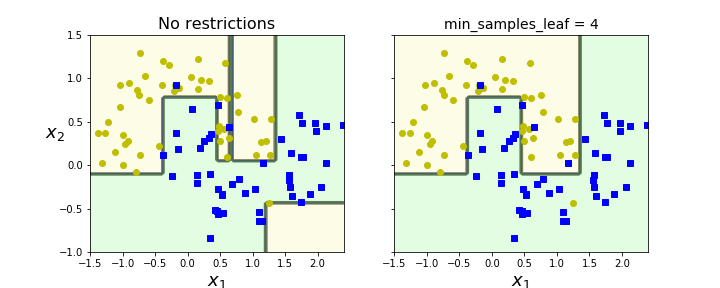
\includegraphics[scale=0.55]{Images/min_samples_leaf_plot.png}
\end{center}

\subsection{Regression}

Decision Trees are capable of performing regression tasks as well. Below we will use Scikit-Learn's \mintinline{python}{DecisionTreeRegressor}
class, training it on a noisy quadratic dataset with a \mintinline{python}{max_depth=2}:

\begin{minted}{python}
from sklearn.tree import DecisionTreeRegressor

# Quadratic training set + noise
np.random.seed(42)
m = 200
X = np.random.rand(m, 1)
y = 4 * (X - 0.5) ** 2
y = y + np.random.randn(m, 1) / 10

tree_reg = DecisionTreeRegressor(max_depth=2, random_state=42)
tree_reg.fit(X, y)
\end{minted}

\noindent
The resulting tree can be seen below:

\begin{center}
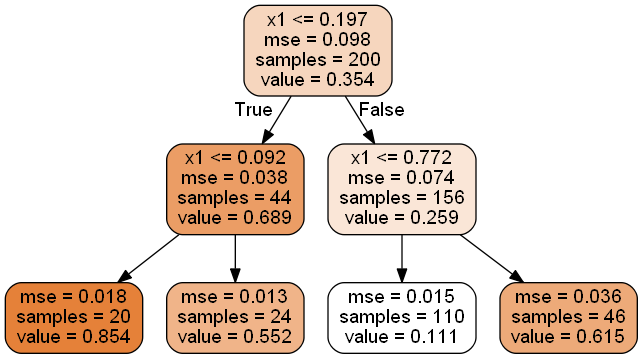
\includegraphics[scale=0.45]{Images/iris_tree_reg.png}
\end{center}

\noindent
We can see that the regression tree looks very similar to the tree that we built earlier. The main difference now is that instead of predicting 
a class in each node, we are now predicting a value instead. Additionally, we can use the same strategy as before when traversing the 
classification based tree (For example, if we wanted to find the node for an input value of $x_{1} = 0.6$). \\

\noindent
This model’s predictions are represented on the left in figure below. If you set \mintinline{python}{max_depth=3}, you get the predictions 
represented on the right. Notice how the predicted value for each region is always the average target value of the instances in that region. 
The algorithm splits each region in a way that makes most training instances as close as possible to that predicted value.

\begin{center}
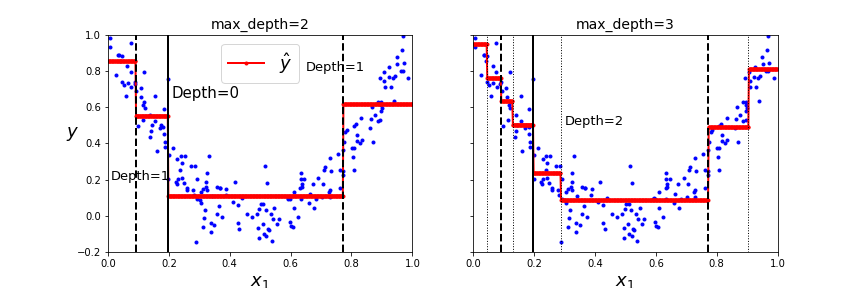
\includegraphics[scale=0.45]{Images/tree_regression_plot.png}
\end{center}

\noindent
The CART algorithm works similarly, except that instead of trying to split the training set in a way that minimizes impurity, it tries to split
the training set in a way that minimizes the \textit{mean squared error} (MSE). Below will be the cost function that the CART algorithm tries
to minimize:

\begin{equation*}   
\begin{aligned}
    \quad & \vec{J}(k, t_{k}) = \frac{m_{left}}{m} \text{MSE}_{left} + \frac{m_{right}}{m} \text{MSE}_{right}\\
\textrm{where} \quad & 
\begin{cases} 
    \text{MSE}_{\text{node}} = \sum_{i \in \text{node}} \left(\hat{y}_{node} - y^{(i)}\right)^{2} \\
    \hat{y}_{\text{node}} = \frac{1}{m_{\text{node}}} \sum_{i \in \text{node}} y^{(i)}
\end{cases}
\end{aligned}
\end{equation*}

\noindent
Additionally, just like classification tasks, Decision Trees are prone to overfitting when dealing with regression tasks. From the figure below
we can see that without any regularization (i.e., using default hyperparameters), we get a model that severely overfits the training data. However,
even just setting \mintinline{python}{min_samples_leaf=10} results in a model that is much more reasonable and looks like it will generalize
much better.

\begin{center}
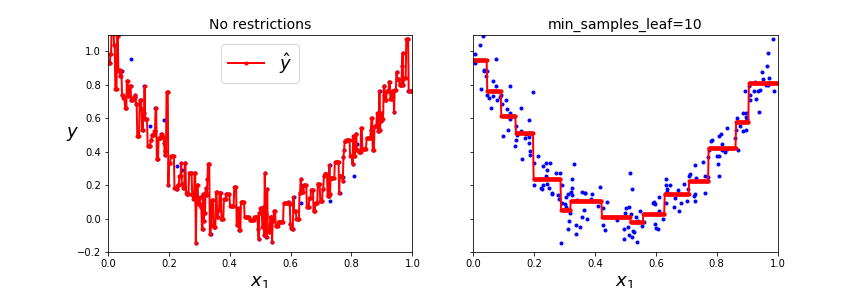
\includegraphics[scale=0.45]{Images/tree_regression_regularization_plot.png}
\end{center}

\subsection{Instability}

Although Decision Trees are a very powerful algorithm, they do have their own limitations. Firstly, Decision Trees tend to use orthogonal
decision boundaries (i.e., splits are perpendicular to an axis), which makes them sensitive to training set rotations. For example, in the 
figure below we can see that the left-hand plot is easily split by a decision tree, however, if we rotate the data 45 degrees, the decision 
boundary looks to be unnecessarily complex. This then causes further issues with the model not being able to generalize well. One thing to fix 
this issue is to use Principal Component Analysis (PCA) which often results in better orientation in the data.

\begin{center}
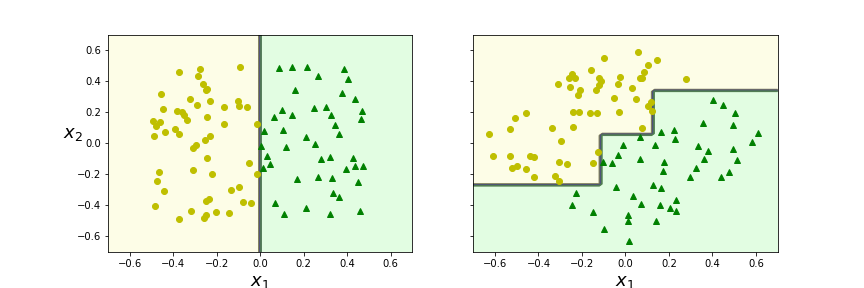
\includegraphics[scale=0.45]{Images/sensitivity_to_rotation_plot.png}
\end{center}

\noindent
However, the main issue with Decision Trees is that they tend to be very sensitive to small variations in the training data. For example, if we 
were to remove the widest \textit{Iris Veriscolor} from the iris training set and train a new Decision Tree, we will get a model that is 
totally different from the model we initially trained. Below will be the plot of the new decision boundaries of the decision tree that does 
not include the widest iris.

\begin{center}
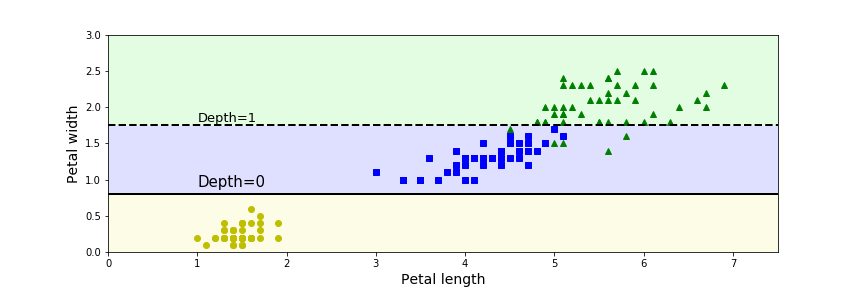
\includegraphics[scale=0.45]{Images/decision_tree_instability_plot.png}
\end{center}

\noindent
As we will see in the next section, Random Forests can limit this instability affect by averaging predictions over many trees.